%!TEX root = project.tex
\subsection{Image Correction}

\begin{figure}[ht]
    \centering
    \begin{minipage}[b]{\figwidth}
        \centering
        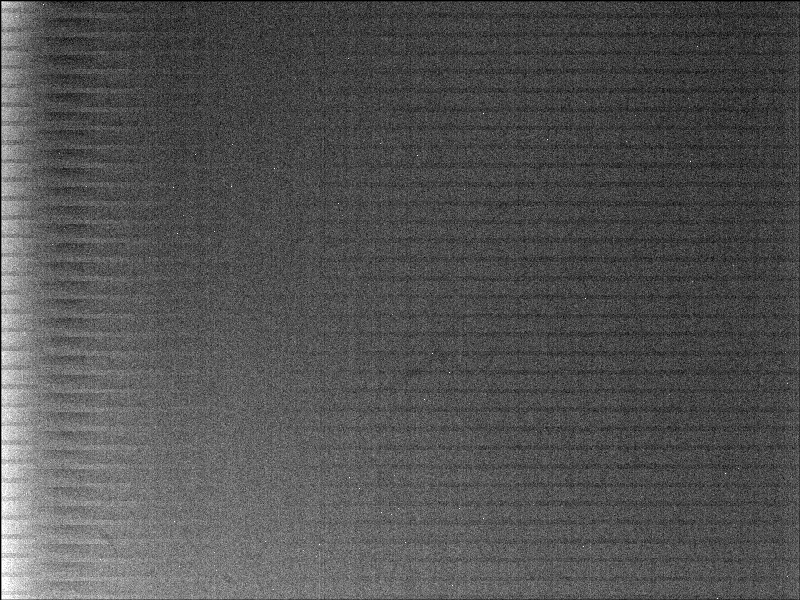
\includegraphics[width=\textwidth]{images/bias.png}
        \caption{Sample bias image generated with our equipment}
        \label{fig:bias_image}
    \end{minipage}\quad\quad
    \begin{minipage}[b]{\figwidth}
        
\includegraphics[width=\textwidth]{images/flat.png}
        \caption{Sample flat image generated with our equipment}
        \label{fig:flat_image}
    \end{minipage}
\end{figure}

\begin{figure}[ht]
    \centering
    \begin{minipage}[b]{\figwidth}
        \centering
        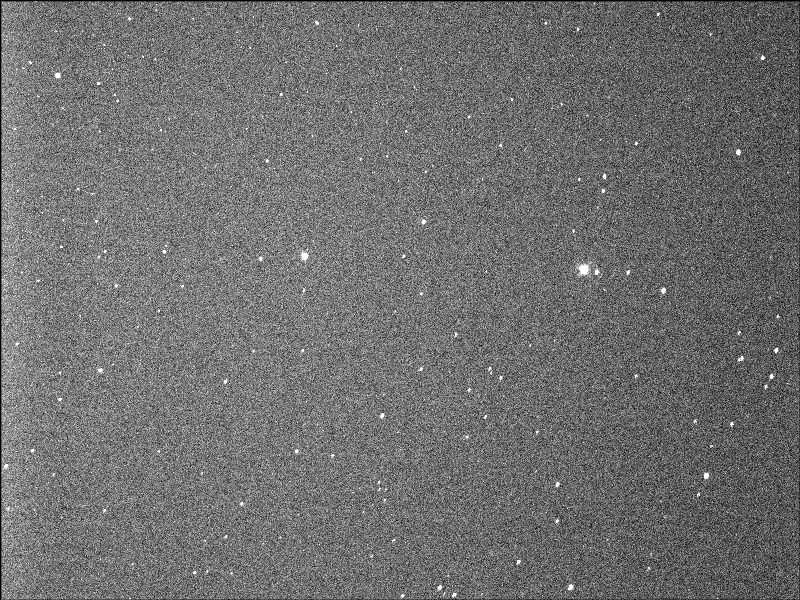
\includegraphics[width=\textwidth]{images/raw_image.png}
        \caption{Uncorrected image from the CCD}
        \label{fig:raw_image}
    \end{minipage}\quad\quad
    \begin{minipage}[b]{\figwidth}
        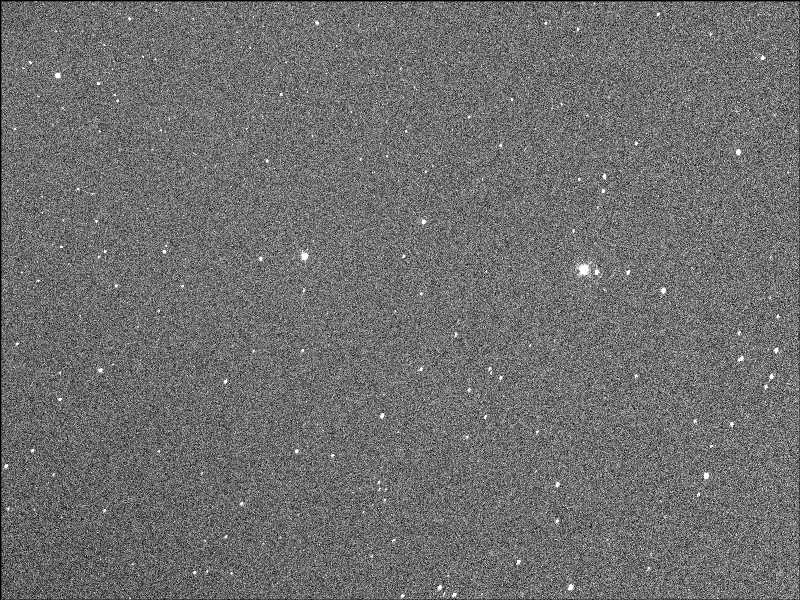
\includegraphics[width=\textwidth]{images/corrected_image.png}
        \caption{Image after applying bias and flat correction}
        \label{fig:corected_image}
    \end{minipage}
\end{figure}

\subsubsection{Bias Image}

Firstly, systematic errors in the optical equipment need to be accounted for. Initially a correction needs to be made for the noise in the CCD electronics. To do this a set of images are taken with the shortest possible exposure time (0 seconds if possible). Then an average is built from this set of images. This data is then subtracted from any image taken using the CCD to get an image without the noise. An example bias image taken with our SBIG CCD can be seen in figure \ref{fig:bias_image}.

\subsubsection{Flat Image}

Secondly, we have to account for varying sensitivity across the CCD. Under normal circumstances, even with an even distribution of light, a CCD will not react perfectly evenly. Essentially there will be a regions of higher and lower sensitivity, and even the best CCD's will have a variation of the order of a few percent. This will have a big impact on our photometry readings as objects move within the frame, as we are looking for flux changes of only a few percent. To correct for this, we take images against a clear patch of sky that will ideally be evenly lit. These images are then averaged. Then, this final average is normalised, and then any image taken by the CCD can be divided by this flat image, after correcting for noise.

\subsubsection{Summary}

So in summary, after creating a bias and a flat image, and image taken by the CCD can be corrected by first substracting the bias image, and secondly dividing by the flat image. Bias and flat images need to be recreated throughout an observing session if possible to compensate for CCD temperature changes. A raw uncorrected image can be seen in figure \ref{fig:raw_image}, and after applying bias and flat correction can be seen again in \ref{fig:corected_image}.

\subsection{Object Detection}

\begin{figure}[ht]
    \centering
    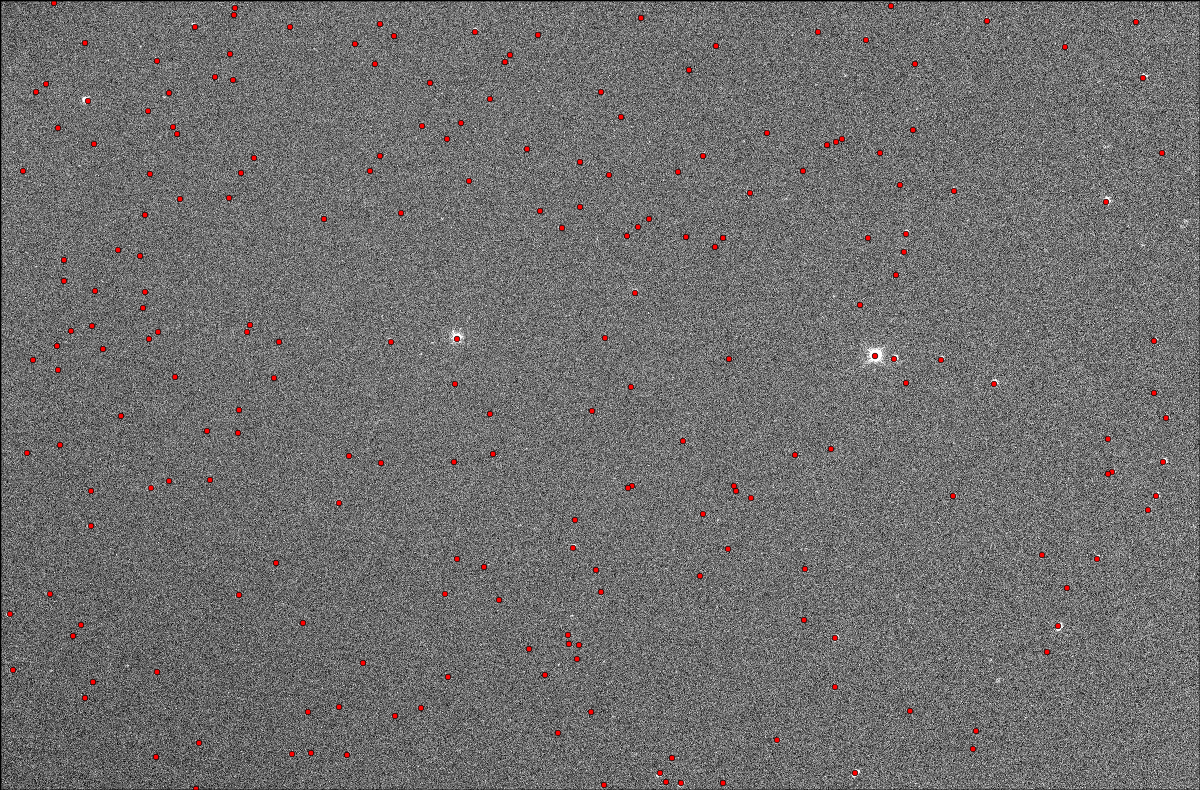
\includegraphics[width=0.85\textwidth]{images/starfinder.png}
    \caption{Corrected image shown with the locations of stars discovered by the software. Red markers show stars found}
    \label{fig:finder_image}
\end{figure}

The first step in performing automated photometry is to actually identify. The common method to find objects in an astronomical image is to use the sextractor tool \citep{bertin1996sextractor}. However as this software is a bit of a black box, I chose to also experiment with writing my own tool to find stars. The pipeline is written to support using both the sextractor tool and my own algorithm interchangeably. Configuration information provided to the sextractor tool can be found in the appendices. An image showing the accuracy of the star finder can be seen in figure \ref{fig:finder_image}.

\subsubsection{Algorithm for star detection}

The algorithm I devised was designed to be as simple as possible, and perform quickly on a large fits images. While code for the algorithm can be found in the listing in the appendix, here is a simple description of the method:
\begin{enumerate}
    \item Estimate the background level
    \item Find local maxima above this background, with SNR above some given threshold
    \item With these maxima locations, perform a 2D gaussian fit around the region to find the center of the object
\end{enumerate}

The final gaussian fit gives both the center of the star with sub pixel accuracy, and a good estimate of the radius of the star by using the FWHM of the gaussian.

\subsection{Object Tracking}

The optical setup and mount alignment are never perfect, so stars will drift inside the field of view. As we are collecting data over a period of the order of around 4 hours for most transitions, stars may have moved by as much as a few hundred pixels between the initial and final image in the sequence.

Objects in the image don't just drift, there will also be some rotation due to imperfect mount alignment. Over the course of an observing session this may be as much as a few degrees. For stars towards the edge of the frame, this could be a large pixel distance on the image.

Luckily, both of these operations are easy to describe mathematically, and thus easy to numerically fit for. Traditionally image transformations in computers are described as a translation, rotation, and scale. In this case, we can disregard any scale change and just concentrate on the translation and rotation transformations.

Rotation is described by the matrix operation:
\[
\begin{bmatrix}
    u \\ v
\end{bmatrix}
=
\begin{bmatrix}
\cos\theta & -\sin\theta \\
\sin\theta & cos\theta
\end{bmatrix}
\begin{bmatrix}
    x \\ y
\end{bmatrix}
\]

The translations is described by:
\[
\begin{bmatrix}
    u \\ v
\end{bmatrix}
=
\begin{bmatrix}
    \Delta x \\ \Delta y
\end{bmatrix} +
\begin{bmatrix}
    x \\ y
\end{bmatrix}
\]

The total change from image to image is then described by the sum of both of these operations. A very simple tracking algorithm can then be constructed by simply using a least squares fit on the data by performing both operations, and attempting to minimise the total pixel difference when subtracting one image from the other. As stars are much brighter than the background, this function will be minimized when the stars lie on top of each other as much as possible. The changes from image to image are small enough so that it doesnt matter which order the operators are applied. For larger drifts this would not be the case as the rotation would no longer be approximately around a fixed point, and a more complex function would be required to describe the change.
\[
\begin{bmatrix}
    u \\ v
\end{bmatrix}
=
\begin{bmatrix}
\cos\theta & -\sin\theta \\
\sin\theta & cos\theta
\end{bmatrix}
\begin{bmatrix}
    x + \Delta x \\ y + \Delta y
\end{bmatrix}
\]

\subsection{Photometry}

To perform photometry, we simply want to calculate the flux of the star. With both a location and estimated radius for the star, this is trivial to obtain. The total flux is simply the sum of the flux inside an aperture with radius of the star, minus the background within the aperture.

\begin{figure}[ht]
    \centering
    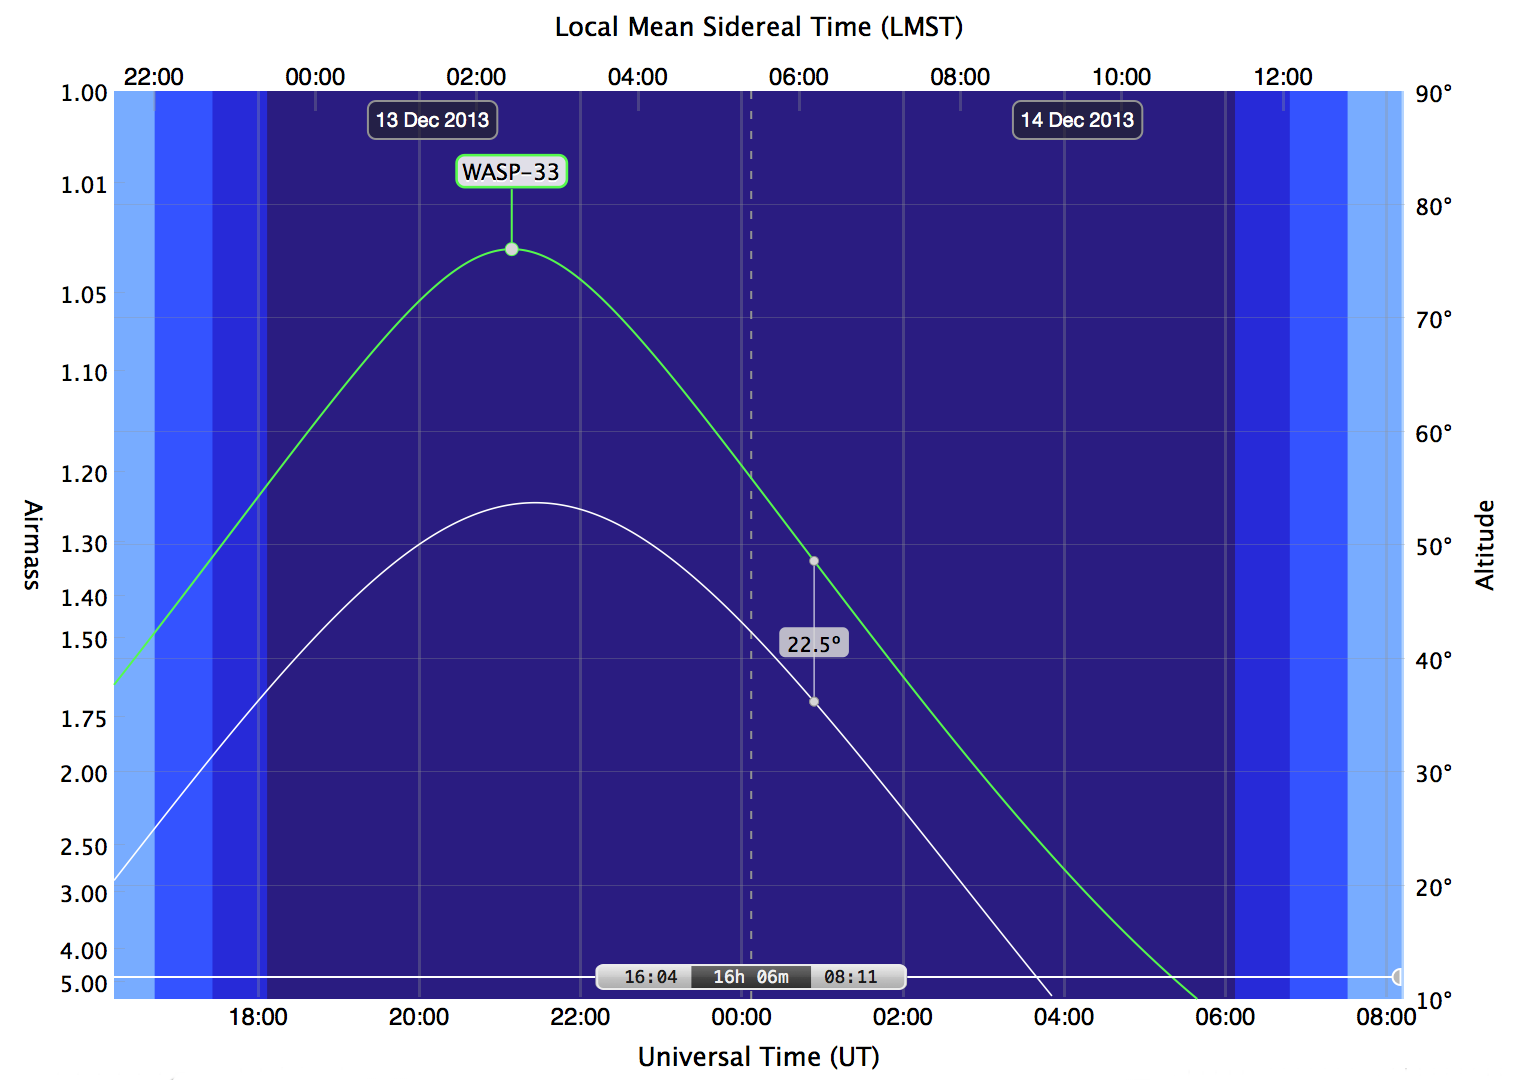
\includegraphics[width=0.85\textwidth]{images/airmass.png}
    \caption{Observational parameters of the star Wasp-33}
    \label{fig:airmass}
\end{figure}

Firstly, an airmass correction can be performed. Most visible transits happen across a range of altitude, and many of the stronger ones are low in the sky. An example of a star with a transit can be seen in figure \ref{fig:airmass}. The airmass can be corrected for simply by normalising for an airmass of one at the zenith, so the airmass is given simply by $\sec \theta$, where $\theta$ is the altitude of the object.

While this gives us flux values for each star, they are not calibrated and so a further calibration step must be performed. This is done by using calibration stars in the same frame, that should be chosen not to be variable.
\[ \text{Calibrated} = \frac{\text{Measured Flux}}{\text{Calibration Star Flux}} \]

This can be performed with many calibration stars to compensate for both not always knowing if a star is a variable, and  differences in seeing across the field of view.